\documentclass{beamer}
\usepackage[utf8]{inputenc}
\usepackage{amsmath,amssymb,bm}
\usepackage{physics}
\usepackage{graphicx}
\usepackage{hyperref}
\usepackage{booktabs}
\usetheme{Madrid}
\usepackage{fontspec}
\usepackage{luatexja-fontspec} % For LuaLaTeX
\setmainjfont{Noto Serif CJK JP}
\usecolortheme{seagull}
\graphicspath{{./}{figures/}{TalksMaterialQML/figures/}{TalksMaterialQML/qcfigures/}}

\title[AI and Quantum Technologies]{\textbf{AI and Quantum Technologies}}
\subtitle{From general considerations to a reinforcement-learning designed quantum sensor}
\author{Morten (\textbf{望天（モーテン）}) Hjorth-Jensen}
\institute[University of Oslo]{Department of Physics and Center for Computing in Science Education, University of Oslo, Norway}
\date{Time and place to be changed}

\begin{document}

%-----------------------------------------------------------
\begin{frame}[plain,fragile]
\titlepage
\end{frame}

\begin{frame}[plain,fragile]
\frametitle{What is this talk about?}
\begin{block}{}
Artificial intelligence and quantum technologies are the two computational revolutions of our time, and they feed each other. The first part of this talk is a pedestrian tour of \emph{why} they are linked. The second part is one concrete example from our own work: how a reinforcement-learning agent can design an entangled quantum sensor made of two electrons floating on liquid helium.
\end{block}
\vspace{3mm}
\begin{block}{Take-home message}
Machine learning is becoming the design and control layer of quantum devices, and quantum devices are becoming new tools for sensing, simulation and, eventually, computing.
\end{block}
\end{frame}

\begin{frame}[plain,fragile]
\frametitle{Thanks to many, and to our sponsors}
{\small
Maria Elena Perruzza (UiA/USN), Niyaz Beysengulov (EeroQ), Stian Bilek, Antoine Camper, Jonas Flaten, Gunnar Lange, Oskar Leinonen, Jan Malamant, Francesco Massel, Heidi Sandaker, Viktor Svensson (UiO), Johannes Pollanen (MSU/EeroQ), Zachary Stewart and Jared Weidman (MSU), and the CERN DRD5 collaboration on quantum sensors.

Jane Kim, Julie Butler, Patrick Cook, Danny Jammooa, Dean Lee, Witek Nazarewicz (MSU), Bryce Fore and Alessandro Lovato (ANL), Giuseppe Carleo (EPFL), Even Nordhagen and Robert Solli (UiO). Excuses to those I have omitted.
}
\vspace{2mm}
\begin{block}{Sponsors}
Research Council of Norway (QONTROL Centre for Quantum Control and other grants), University of Oslo, and earlier support from NSF and DOE (US) and Michigan State University.
\end{block}
\end{frame}

\begin{frame}[plain,fragile]
\frametitle{Outline}
\tableofcontents
\end{frame}

%-----------------------------------------------------------
\section{Two revolutions and why they meet}

\begin{frame}[plain,fragile]
\frametitle{Quantum technology and machine learning/AI}
\centerline{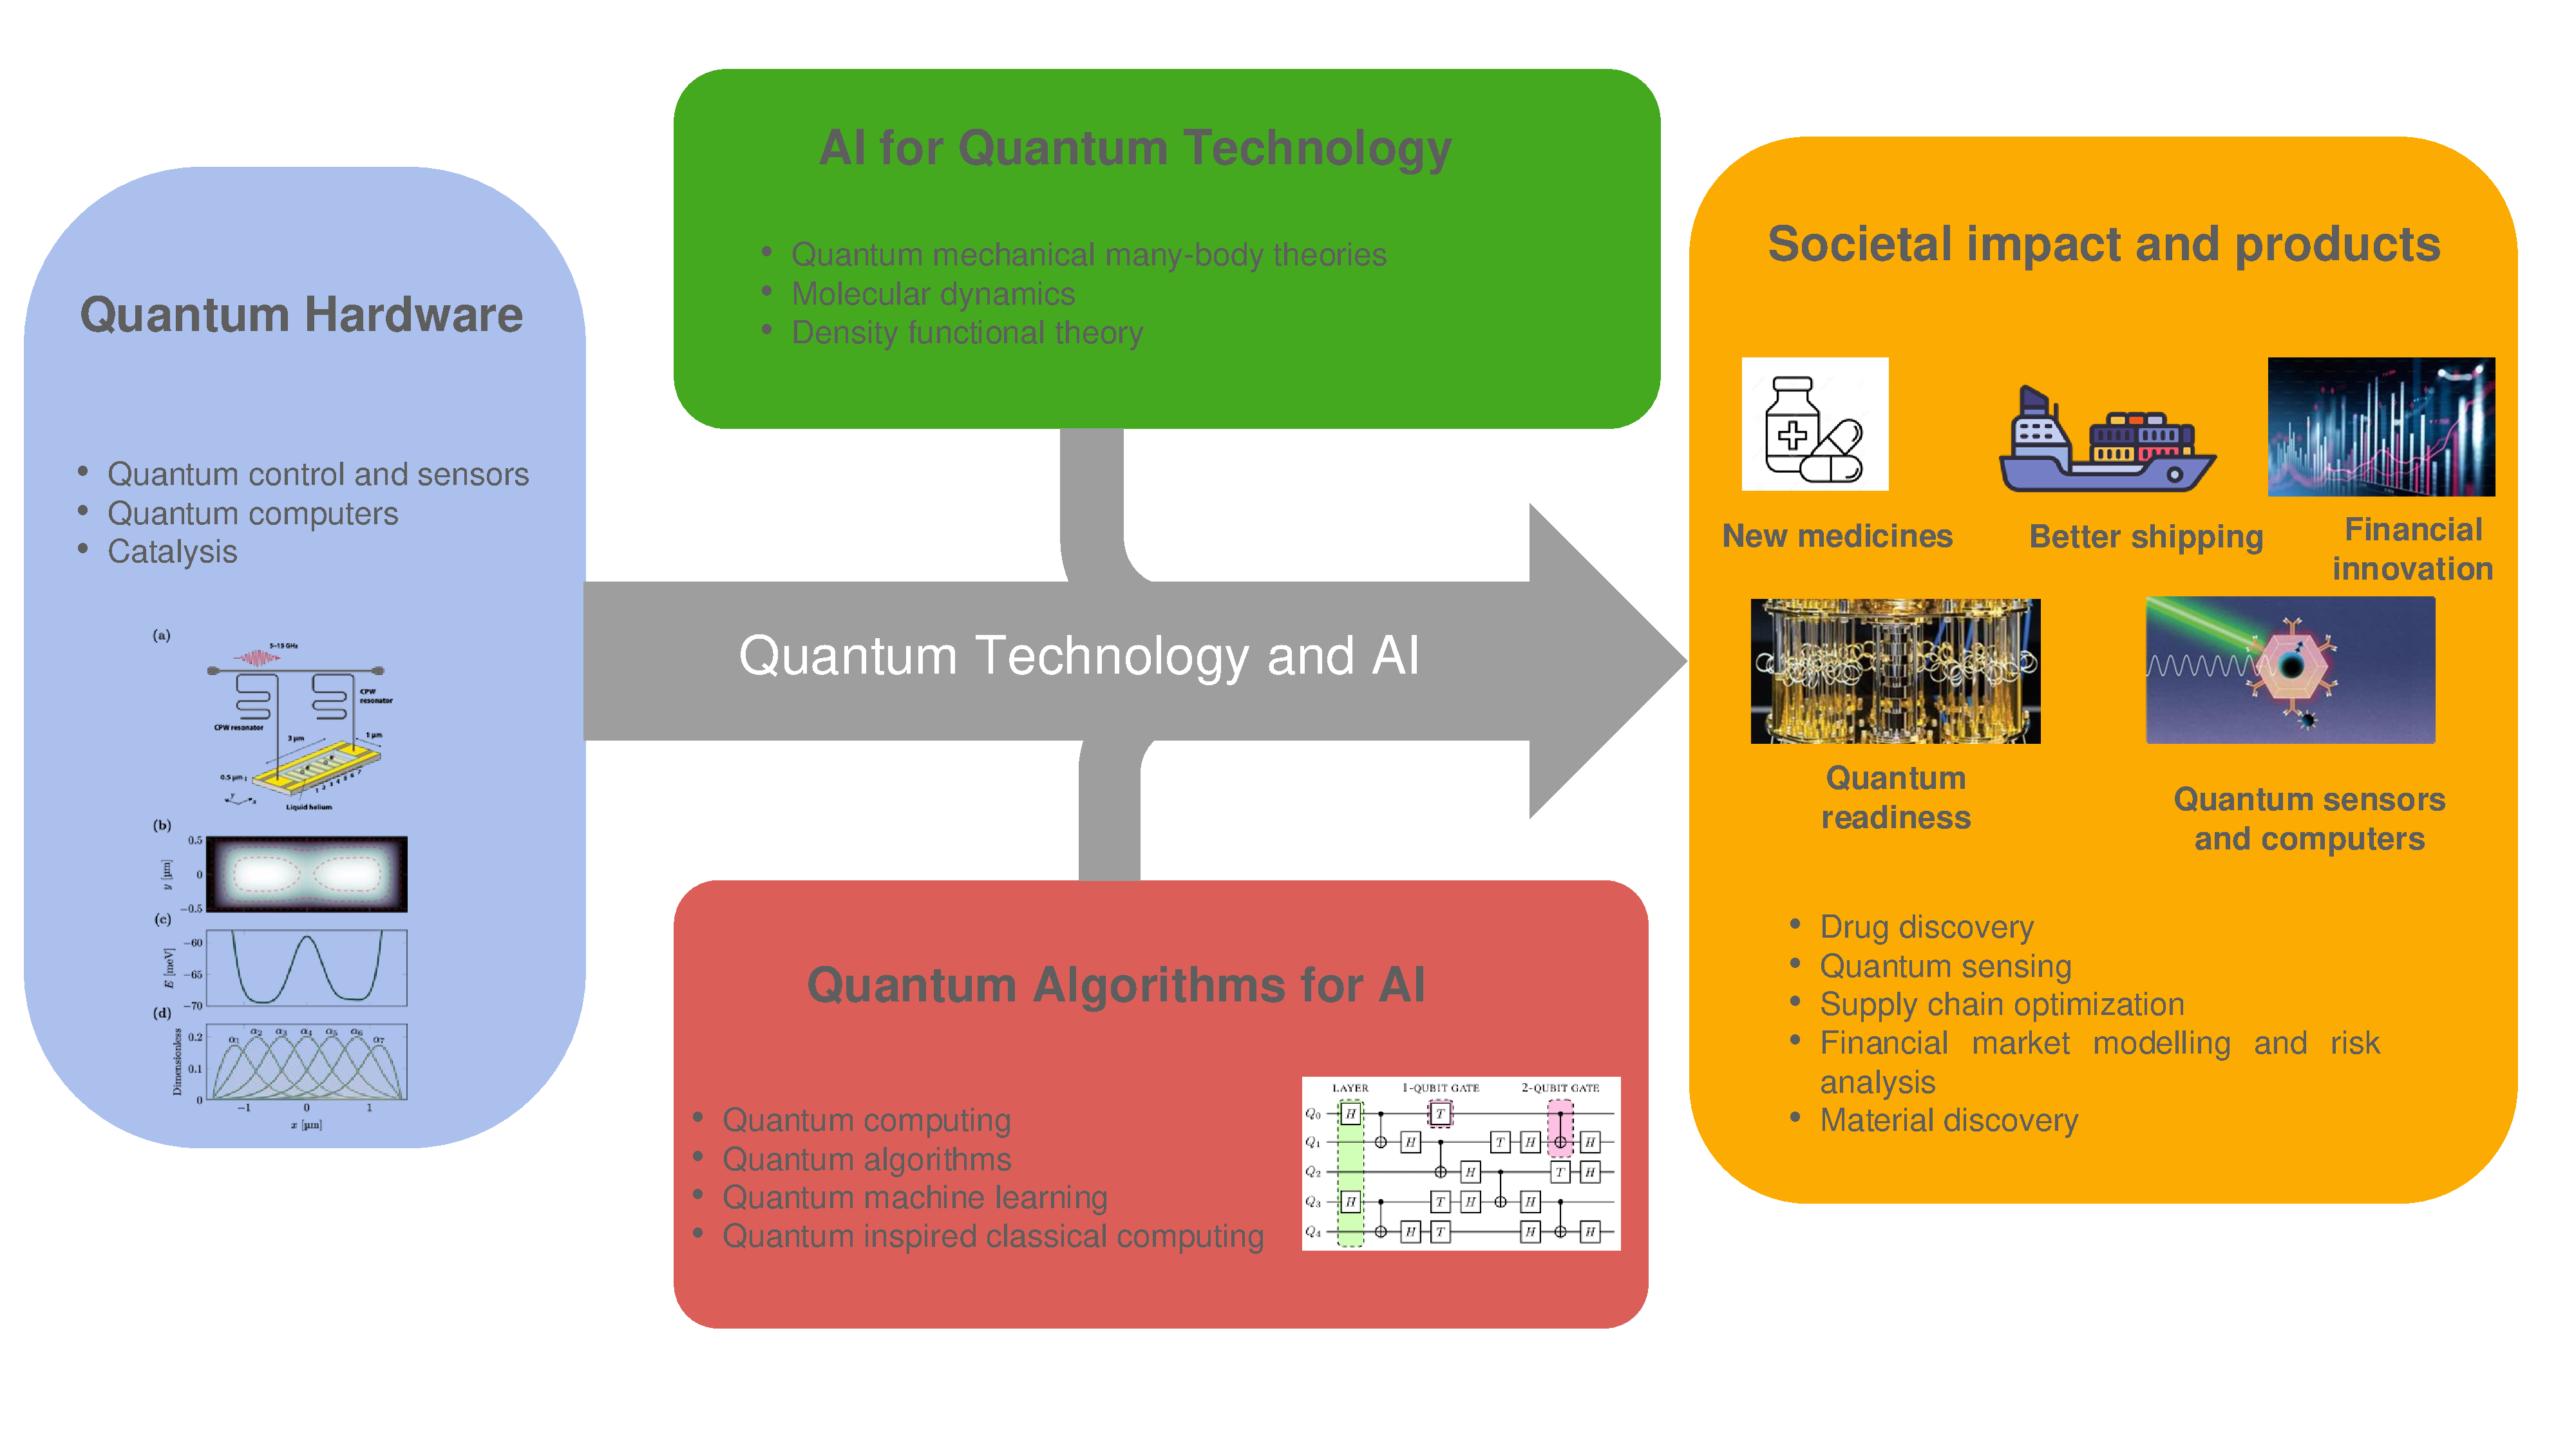
\includegraphics[width=1.0\linewidth]{figureintro.pdf}}
\end{frame}

\begin{frame}[plain,fragile]
\frametitle{What do we mean by AI and machine learning?}
\begin{block}{}
Here: a collection of methods that \textbf{learn a model from data by minimising a cost function}. At the heart of every machine-learning method there is an optimisation problem.
\end{block}
\begin{itemize}
\item \textbf{Supervised learning:} labelled data, regression and classification.
\item \textbf{Unsupervised learning:} find structure without labels (clustering, dimensionality reduction, generative models).
\item \textbf{Reinforcement learning (RL):} an \emph{agent} acts on an \emph{environment}, receives a \emph{reward}, and learns a policy that maximises it.
\end{itemize}
\[
\text{data } \bm{x} \;\rightarrow\; \text{model } f_{\bm{\theta}} \;\rightarrow\; \text{cost } \mathcal{C}(\bm{x},f_{\bm{\theta}}) \;\rightarrow\; \min_{\bm{\theta}} \mathcal{C}
\]
The third family is the one we will use later: a physics simulator is the environment, electrode voltages are the actions, and the reward is a measure of sensor quality.
\end{frame}

\begin{frame}[plain,fragile]
\frametitle{What do we mean by quantum technologies?}
Devices whose function relies on \textbf{superposition}, \textbf{entanglement} and \textbf{interference} of well-controlled quantum states,
\[
\ket{\psi}=\alpha\ket{0}+\beta\ket{1},\qquad
\ket{\Phi^+}=\frac{1}{\sqrt{2}}\left(\ket{00}+\ket{11}\right).
\]
\begin{enumerate}
\item \textbf{Quantum computing and simulation:} qubits and gates; Hilbert space grows as $2^N$.
\item \textbf{Quantum communication and cryptography:} security from physics, not from computational hardness.
\item \textbf{Quantum sensing and metrology:} entangled probes beat the shot-noise limit.
\end{enumerate}
\begin{block}{}
Platforms: superconducting circuits, trapped ions, neutral atoms, photons, spins in semiconductors, and, our favourite, \textbf{electrons on liquid helium}.
\end{block}
\end{frame}

\begin{frame}[plain,fragile]
\frametitle{Quantum sensing in one slide}
Estimate a parameter $\varphi$ (a field, a phase, a frequency) encoded in a quantum state $\ket{\psi(\varphi)}$.
\begin{itemize}
\item $N$ independent probes: standard quantum limit $\Delta\varphi \sim 1/\sqrt{N}$.
\item $N$ entangled probes: Heisenberg limit $\Delta\varphi \sim 1/N$.
\end{itemize}
The precision is bounded by the quantum Cram\'er--Rao bound and the quantum Fisher information $F_Q$,
\[
\mathrm{Var}(\varphi_{\rm est}) \ge \frac{1}{\nu F_Q(\varphi)},
\]
with, for a pure state,
\[
F_Q = 4\left[\braket{\partial_\varphi\psi|\partial_\varphi\psi}-\left|\braket{\psi|\partial_\varphi\psi}\right|^2\right].
\]
\begin{block}{}
Entanglement is a \emph{resource}: it increases the variance of the generator that imprints $\varphi$, and hence $F_Q$. Differential (singlet) probes also reject common-mode noise.
\end{block}
{\footnotesize Degen, Reinhard, Cappellaro, Rev.\ Mod.\ Phys.\ \textbf{89}, 035002 (2017).}
\end{frame}

\begin{frame}[plain,fragile]
\frametitle{Why do AI and quantum technologies need each other?}
\begin{columns}
\column{0.5\linewidth}
\begin{block}{AI for quantum}
\begin{itemize}
\item Device design and optimisation of control pulses and gate voltages
\item Calibration, readout classification, error mitigation and decoding
\item Neural-network quantum states for many-body simulation
\end{itemize}
\end{block}
\column{0.5\linewidth}
\begin{block}{Quantum for AI}
\begin{itemize}
\item Quantum machine learning: variational circuits, kernels
\item Quantum simulators as data generators for hard physics
\item Energy: can quantum hardware reduce the cost of some computations?
\end{itemize}
\end{block}
\end{columns}
\vspace{3mm}
\begin{block}{Common ground}
Both are optimisation problems in exponentially large spaces; both need physicists who speak both languages.
\end{block}
\end{frame}

\begin{frame}[plain,fragile]
\frametitle{AI as a tool for quantum engineering}
\centerline{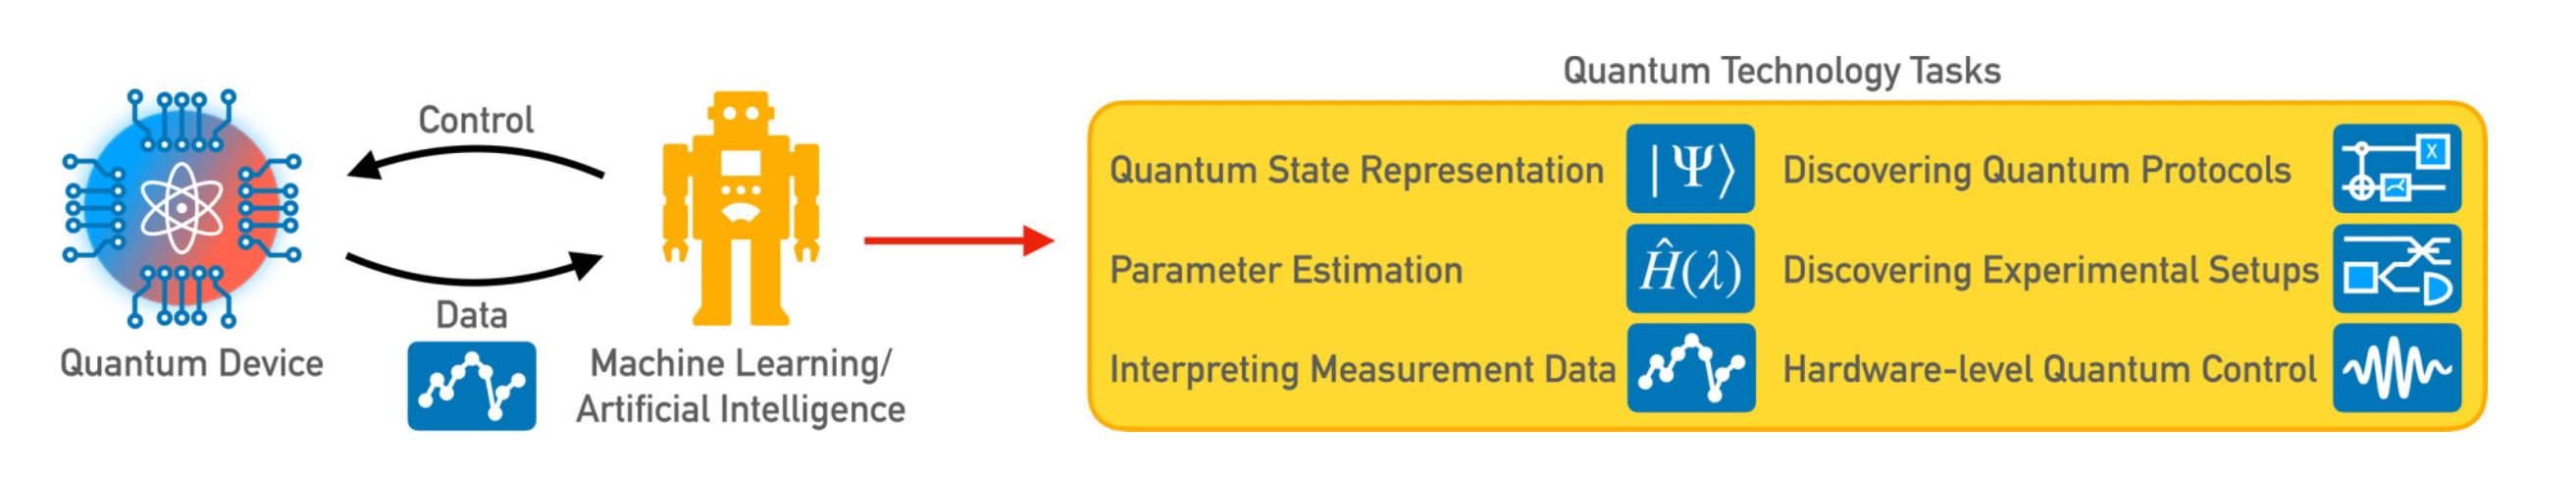
\includegraphics[width=1.0\linewidth]{krenn1.png}}
{\footnotesize Machine learning enters at every stage: design of experiments, control, characterisation, and discovery of new protocols.}
\end{frame}

\begin{frame}[plain,fragile]
\frametitle{AI as a tool for quantum many-body physics}
\begin{columns}
\column{0.55\linewidth}
\centerline{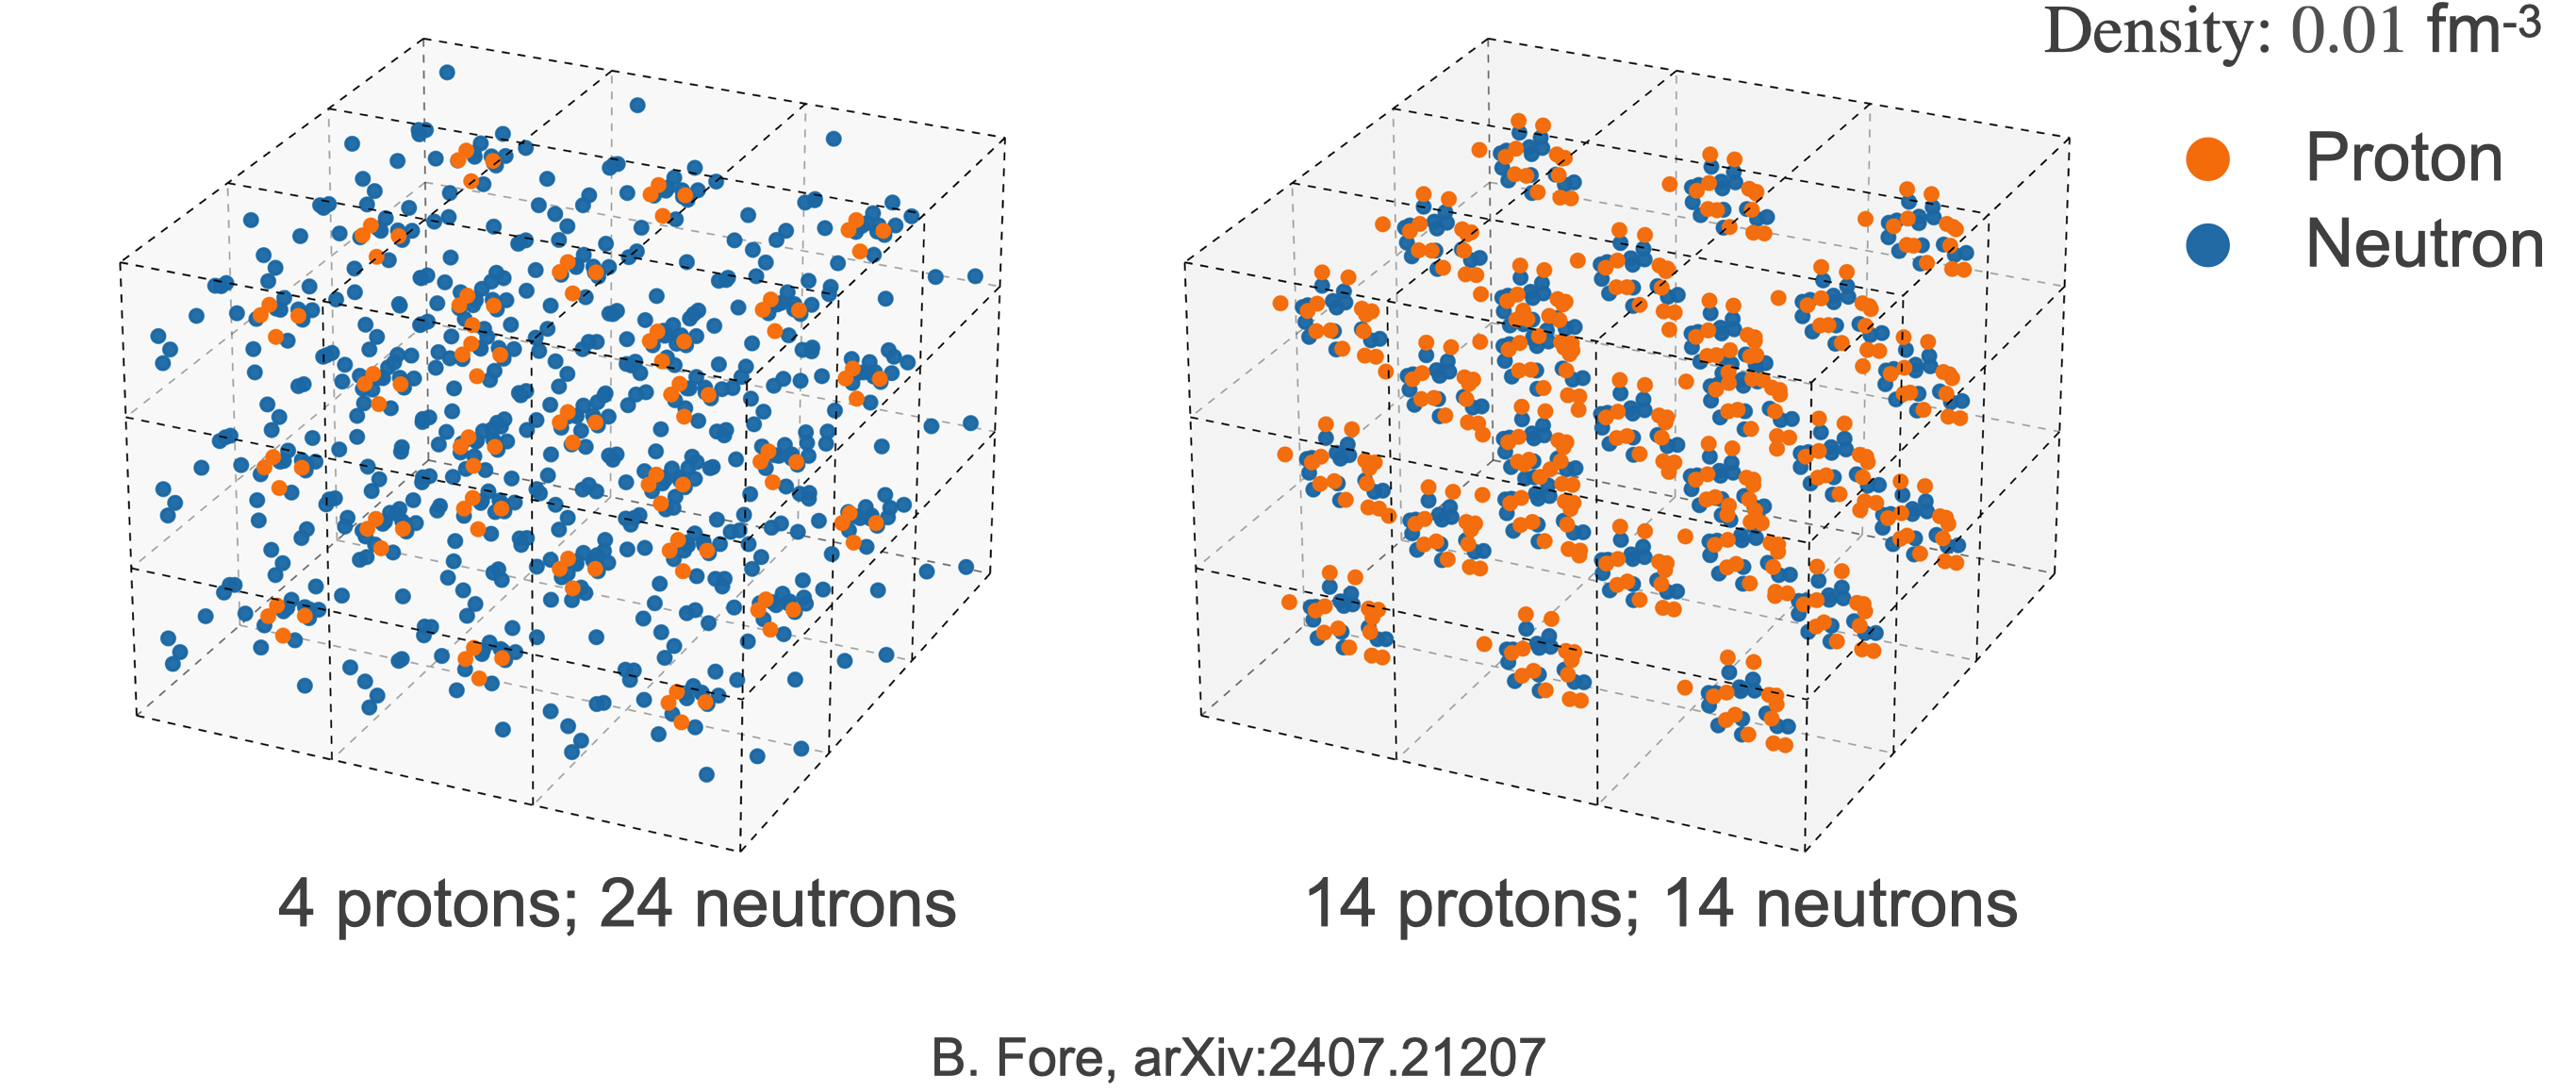
\includegraphics[width=1.0\linewidth]{mbpfig7.png}}
\column{0.45\linewidth}
\begin{itemize}
\item Neural-network quantum states solve the many-body Schr\"odinger equation variationally
\item Self-emerging clustering in the crust of neutron stars
\item Same ideas apply to electrons in quantum dots and on helium
\end{itemize}
\end{columns}
{\footnotesize Fore, Kim, Hjorth-Jensen, Lovato, Communications Physics \textbf{8}, 108 (2025).}
\end{frame}

%-----------------------------------------------------------
\section{An example: a reinforcement-learning designed quantum sensor}

\begin{frame}[plain,fragile]
\frametitle{Electrons on liquid helium as a quantum platform}
\begin{columns}
\column{0.55\linewidth}
\centerline{
\includegraphics[width=1.0\linewidth]{fig1.pdf}}
\column{0.45\linewidth}
\begin{itemize}
\item Electron floats in vacuum above a superfluid helium film: no lattice, no nuclear spins, no defects
\item Predicted spin coherence times of seconds or more
\item Electrodes below the helium shape a \textbf{double-well trap}; each electron couples to a microwave cavity
\item Single-electron trapping and strong cavity coupling demonstrated experimentally
\end{itemize}
\end{columns}
{\footnotesize Panels (b),(c): gate geometries of Castoria et al.\ (2025) and Koolstra et al.\ (2026). Theory: Beysengulov et al., PRX Quantum \textbf{5}, 030324 (2024); Leinonen et al.\ (2025).}
\end{frame}

\begin{frame}[plain,fragile]
\frametitle{The idea: an entangled pair as a differential sensor}
Two electrons, one in each well, prepared in the spin singlet
\[
\ket{S}=\frac{1}{\sqrt{2}}\left(\ket{\uparrow_L\downarrow_R}-\ket{\downarrow_L\uparrow_R}\right).
\]
\begin{itemize}
\item A \textbf{uniform} field shifts both spins equally: the singlet does not care.
\item A \textbf{difference} $\delta B=B_L-B_R$ between the wells couples the singlet to the triplet $\ket{T_0}$: the state starts to oscillate.
\item The pair is a noise-cancelling magnetometer, sensitive to a localised perturbation, for instance from a passing particle or a weak exotic field.
\end{itemize}
\begin{block}{Context}
Proposed in line with CERN's Detector R\&D initiative on quantum sensors (DRD5): rare, sub-keV events, ultralight dark-matter candidates, transient fields.
\end{block}
\end{frame}

\begin{frame}[plain,fragile]
\frametitle{The physics model, in two equations}
Two interacting electrons in a two-dimensional trap ($\hbar^2/2m_e=1$),
\[
\hat{H} = \sum_{i=1}^{2} \left( -\frac{1}{2}\nabla_i^2 + v(\bm{r}_i) \right) + \frac{\kappa}{\sqrt{|\bm{r}_1-\bm{r}_2|^2+\epsilon^2}} .
\]
\begin{itemize}
\item $v(\bm{r})$: electrostatic potential set by four electrode voltages $V=\{V_{\rm unload},V_{\rm trap},V_{\rm res},V_{\rm barrier}\}$.
\item One-body problem on a discrete-variable-representation grid; localised orbitals L0, L1, \dots and R0, R1, \dots by projecting on each well.
\item Two-body problem by \textbf{full configuration interaction}: exact singlet and triplet states in the truncated basis.
\end{itemize}
A magnetic-field gradient enters through
\[
H_B = g\mu_B \bar{B}\,(S^z_L+S^z_R) + \frac{g\mu_B\,\delta B}{2}\,(S^z_L-S^z_R),\qquad
\bra{T_0}H_B\ket{S}=\frac{g\mu_B\,\delta B}{2}.
\]
\end{frame}

\begin{frame}[plain,fragile]
\frametitle{How the signal is read out and how good it can be}
Prepare the singlet-like ground state $\ket{g}$, wait a time $t$, measure the triplet-like population:
\[
P_{g\to e}(t)=\frac{4\lambda^2}{\Delta_{ST}^2+4\lambda^2}\sin^2\!\left[\frac{t}{2\hbar}\sqrt{\Delta_{ST}^2+4\lambda^2}\right],\qquad
\lambda=\frac{g\mu_B\,\delta B}{2}\,\mathcal{M}_{ge}.
\]
\begin{itemize}
\item $\Delta_{ST}$: singlet--triplet splitting; $\mathcal{M}_{ge}=\bra{e}S^z_L-S^z_R\ket{g}$, equal to 1 for a perfect L0--R0 pair.
\item Quantum Fisher information at short times: $F_Q^{ST}\simeq |\mathcal{M}_{ge}|^2 \left(g\mu_B t/\hbar\right)^2$.
\item Two \emph{independent} spins (Ramsey benchmark): $F_Q^{\rm ind}=\tfrac12\left(g\mu_B t/\hbar\right)^2$.
\end{itemize}
\begin{block}{}
The ideal entangled pair gives \textbf{twice} the Fisher information of two independent probes. Everything that degrades the double well (leakage, delocalised orbitals, charge admixture) shrinks $|\mathcal{M}_{ge}|^2$.
\end{block}
\end{frame}

\begin{frame}[plain,fragile]
\frametitle{Where AI enters: let an agent design the trap}
\begin{columns}
\column{0.5\linewidth}
\begin{block}{The RL problem}
\begin{itemize}
\item \textbf{Environment:} DVR + CI solver, time evolution under $\delta B$, Fisher information
\item \textbf{Action:} the four electrode voltages
\item \textbf{Reward:} sensor quality
\item \textbf{Agent:} actor--critic network trained with Proximal Policy Optimisation (PPO), one-shot episodes
\end{itemize}
\end{block}
\column{0.5\linewidth}
\begin{block}{The reward}
\[
R(\bm{a}) = r_{\rm f}\, r_{\rm cfi} - \left(\omega_\mu p_\mu + \omega_{\rm b} p_{\rm b}\right)
\]
\begin{itemize}
\item $r_{\rm f}=F_{\rm singlet}F_{\rm triplet}$: fidelities of ground and first excited state
\item $r_{\rm cfi}$: classical Fisher information of the two- and three-channel readouts
\item penalties for delocalised orbitals and for a barrier that is too low
\end{itemize}
\end{block}
\end{columns}
{\footnotesize PPO: Schulman et al.\ (2017); RL for metrology: Belliardo et al.\ (2024), Bukov et al.\ (2026).}
\end{frame}

\begin{frame}[plain,fragile]
\frametitle{What the agent found: a clean double well}
\centerline{
\includegraphics[width=1.0\linewidth]{fig2.pdf}}
{\footnotesize Left: two-dimensional potential (eV) for the RL-optimised voltages. Right: cut along the red dashed line ($y\approx-0.125\,\mu$m). Wells about $1.5\,\mu$m apart, level spacings of 5--15 GHz.}
\end{frame}

\begin{frame}[plain,fragile]
\frametitle{\ldots with well-localised orbitals}
\centerline{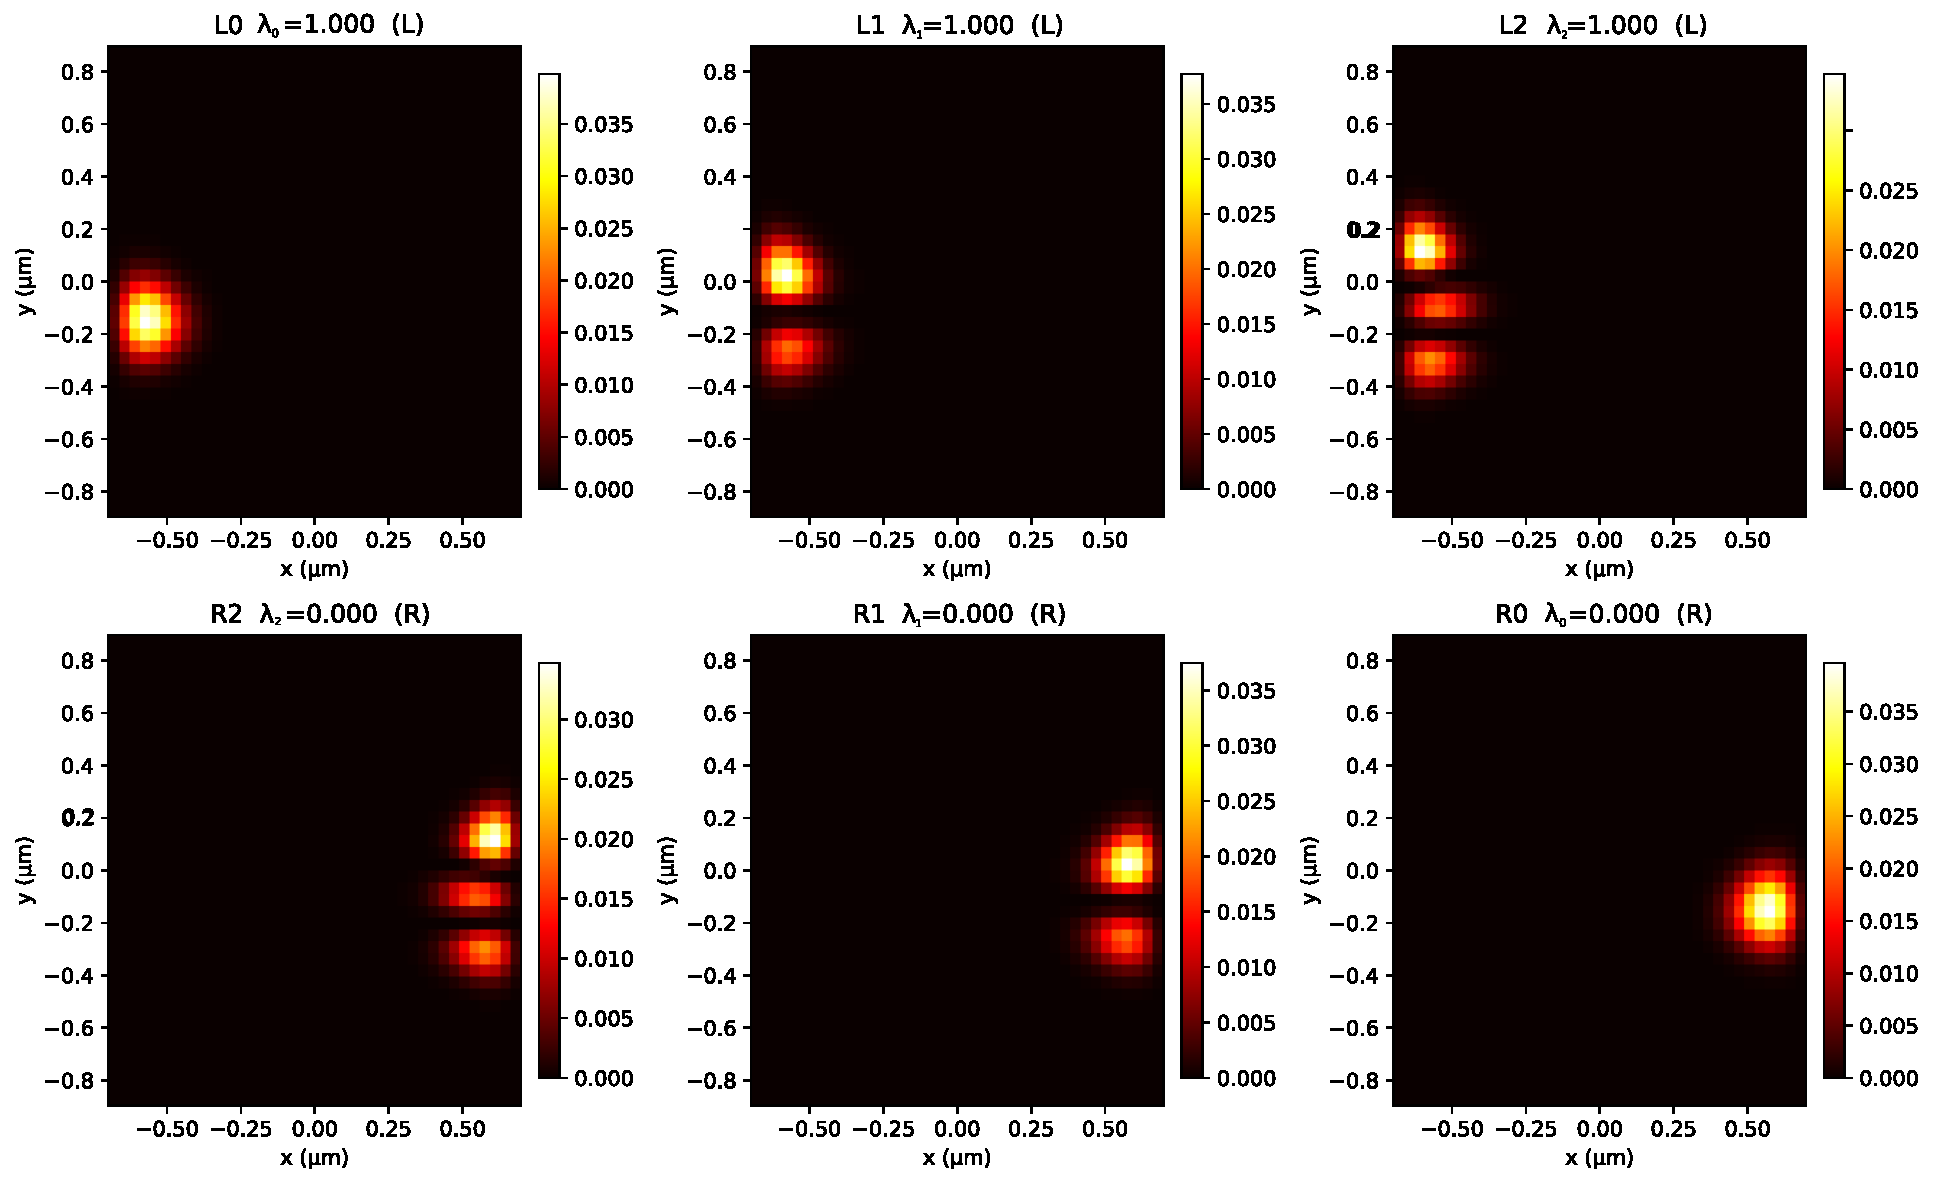
\includegraphics[width=0.95\linewidth]{fig3.pdf}}
{\footnotesize One-body probabilities of the three lowest left-localised (L0, L1, L2, top) and right-localised (R0, R1, R2, bottom) orbitals. Localisation is what makes $\ket{00}=\ket{0}_L\otimes\ket{0}_R$ a good qubit pair.}
\end{frame}

\begin{frame}[plain,fragile]
\frametitle{Sensing dynamics: the two-level picture holds}
\centerline{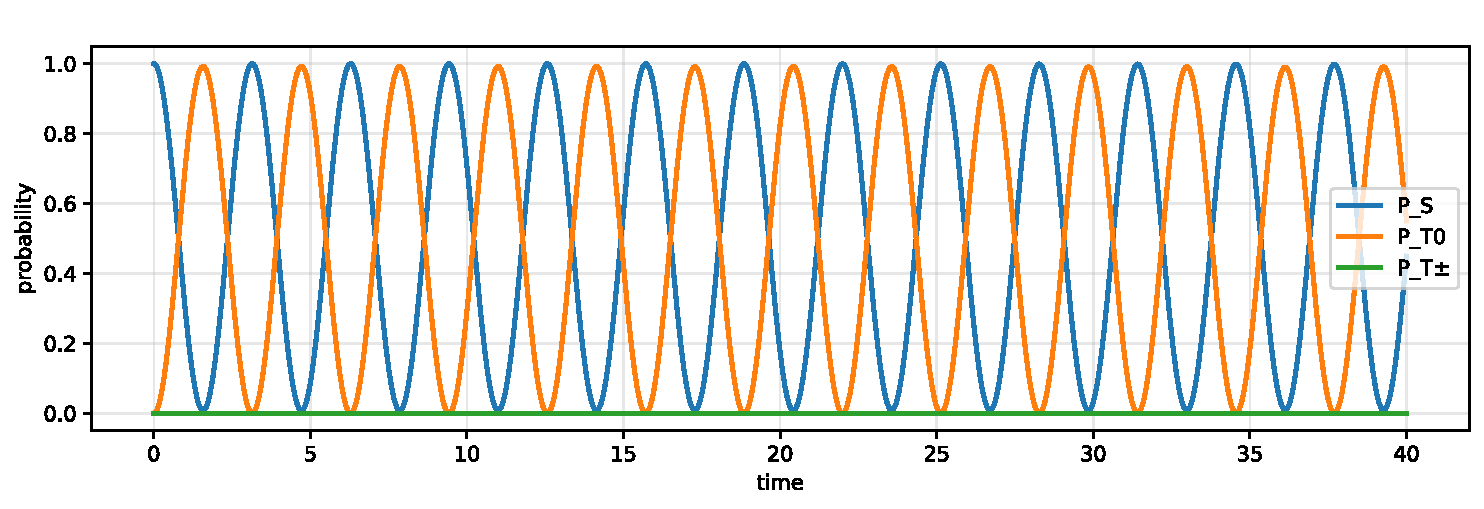
\includegraphics[width=0.9\linewidth]{fig4.pdf}}
{\footnotesize Populations of $\ket{S^*}$, $\ket{T_0^*}$ and $\ket{T_\pm^*}$ under a field gradient for the RL-optimised trap. The full CI dynamics is well described by the effective singlet--triplet Hamiltonian. Time in units of $\mu$m$^2$ ($\hbar=1$).}
\end{frame}

\begin{frame}[plain,fragile]
\frametitle{Fisher information: entangled probe versus independent spins}
\begin{columns}
\column{0.5\linewidth}
\centerline{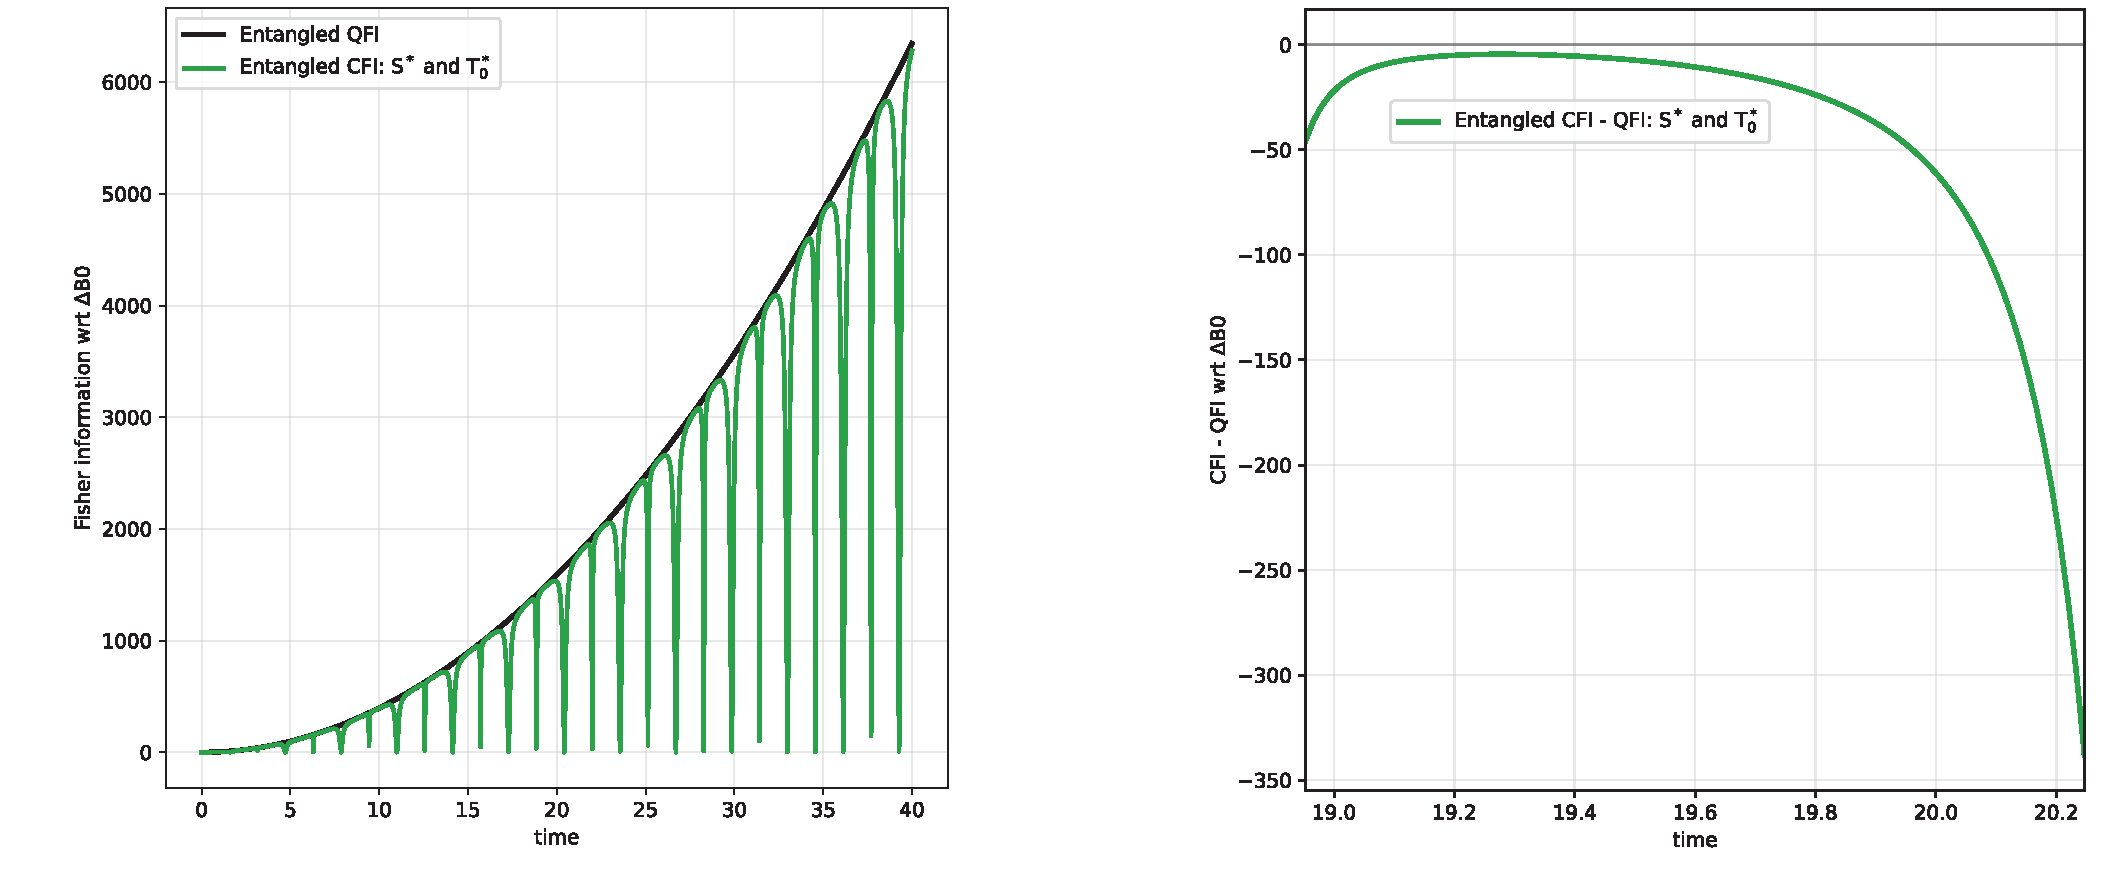
\includegraphics[width=1.0\linewidth]{fig5.pdf}}
{\footnotesize Entangled probe: quantum (QFI) and classical (CFI) Fisher information.}
\column{0.5\linewidth}
\centerline{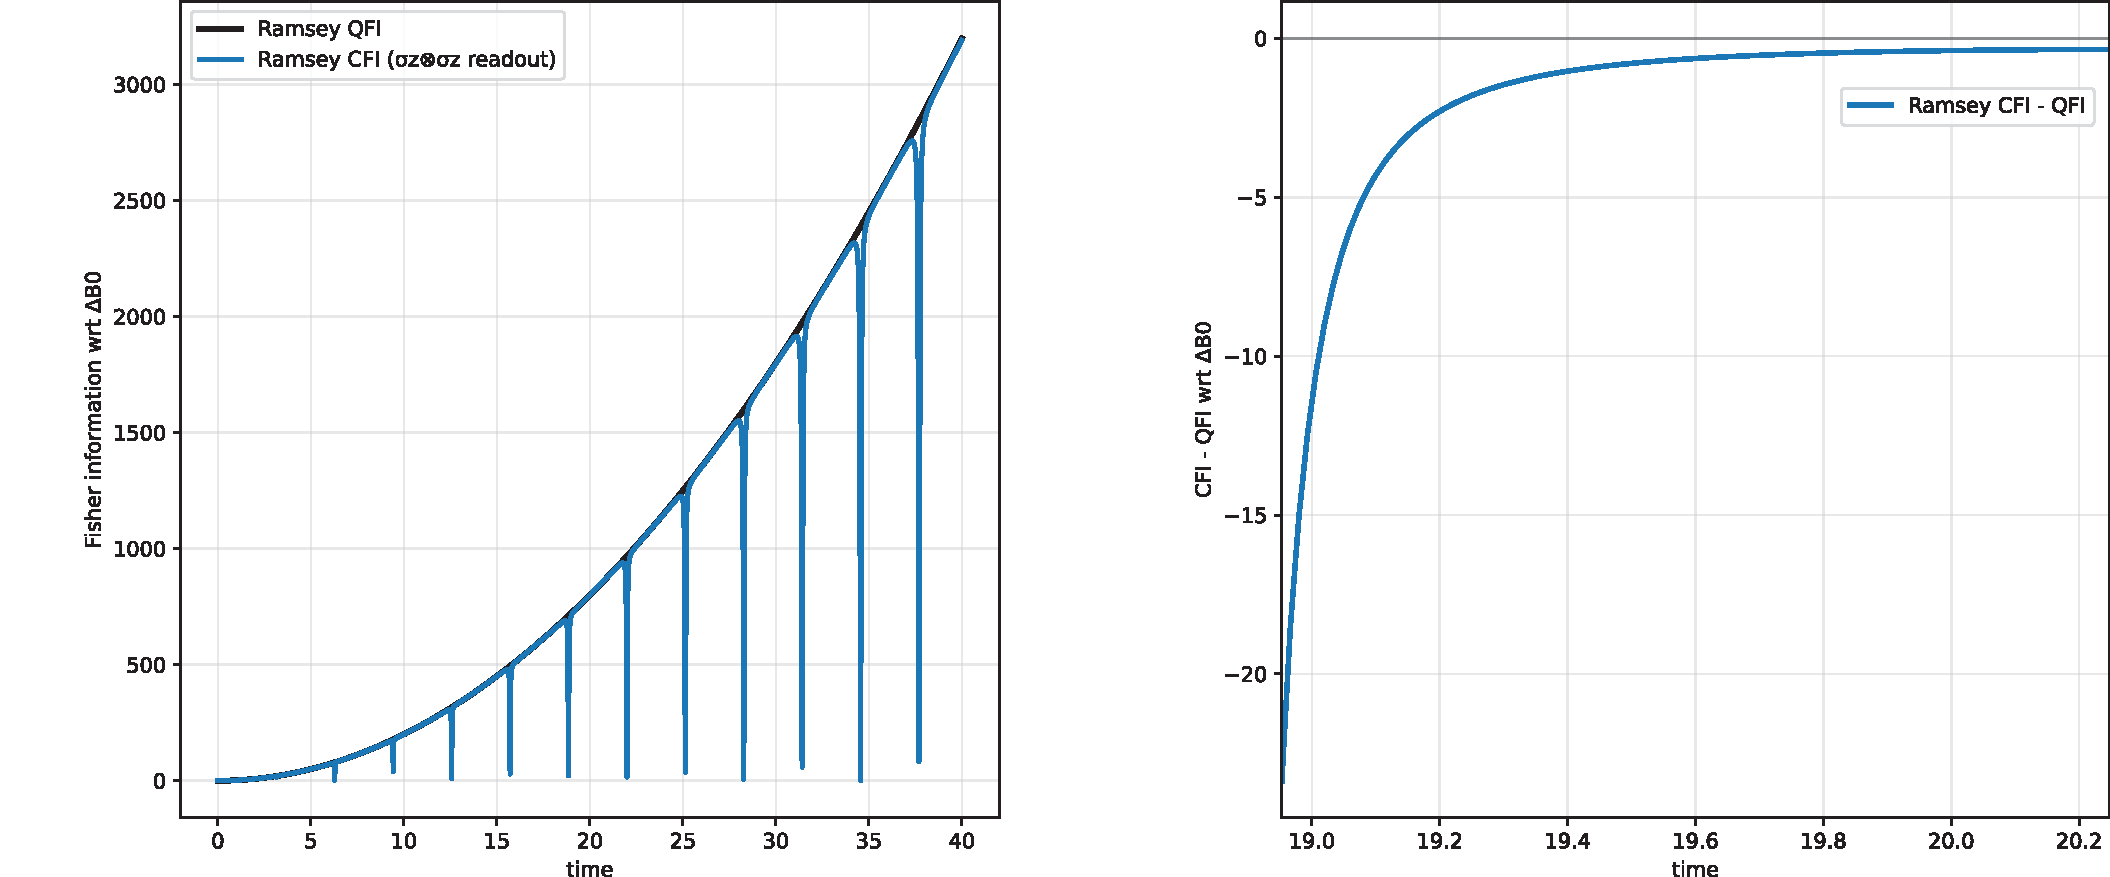
\includegraphics[width=1.0\linewidth]{fig6.pdf}}
{\footnotesize Independent-spin Ramsey benchmark: half the Fisher information.}
\end{columns}
\begin{itemize}
\item The classical Fisher information saturates the quantum bound except at interrogation times where $\partial_{\delta B}P_{g\to e}=0$ (the dips).
\item In the optimal regime the entangled protocol reaches twice the Ramsey benchmark, within 1\%.
\end{itemize}
\end{frame}

\begin{frame}[plain,fragile]
\frametitle{The factor of two is robust in time}
\centerline{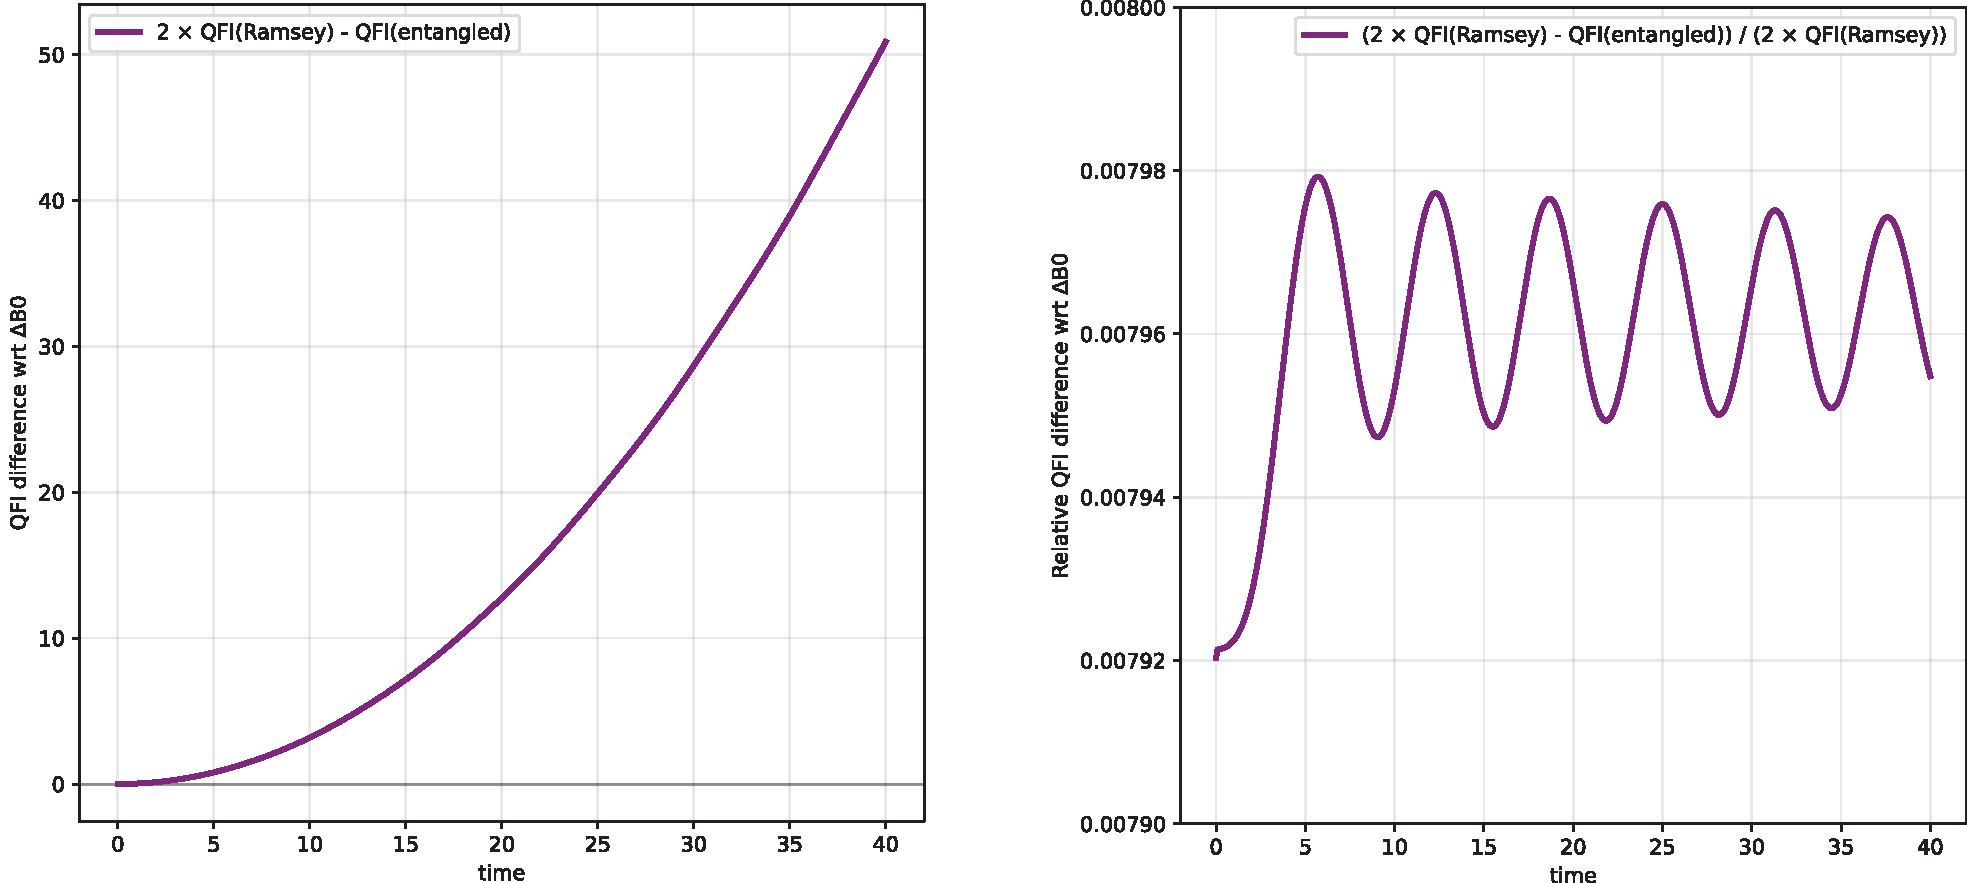
\includegraphics[width=0.9\linewidth]{fig7.pdf}}
{\footnotesize Absolute (left) and relative (right) difference between $2\times$QFI(Ramsey) and QFI(entangled). The relative difference stays constant within an envelope. Static field gradient only; time-dependent fields are future work.}
\end{frame}

\begin{frame}[plain,fragile]
\frametitle{From two qubits to a sensor network, and the hard parts}
\begin{columns}
\column{0.5\linewidth}
\begin{block}{Scaling up}
\begin{itemize}
\item Arrays of coupled electrons: collective response, $F_Q\propto N^2$
\item Singlets for gradients (local events), GHZ-type states for common-mode fields (oscillating backgrounds)
\item Same RL machinery can design the array
\end{itemize}
\end{block}
\column{0.5\linewidth}
\begin{block}{Challenges}
\begin{itemize}
\item Millikelvin cryogenics and superfluid helium handling
\item Single-electron spin readout: spin-to-charge conversion, quantum-limited amplifiers
\item Fabrication uniformity across many traps
\item Coupling the signal in without letting the noise in
\end{itemize}
\end{block}
\end{columns}
\vspace{2mm}
\begin{block}{}
This is a theoretical proposal: the physics is solved exactly for two electrons, the experiments so far characterise single electrons.
\end{block}
\end{frame}

%-----------------------------------------------------------
\section{Conclusions and perspectives}

\begin{frame}[plain,fragile]
\frametitle{Observations (or conclusions if you prefer)}
\begin{block}{}
\begin{itemize}
\item Quantum sensing is where quantum technologies may pay off first, and entanglement gives a quantifiable gain: here a factor of two in Fisher information for a two-electron probe.
\item Machine learning is the natural \textbf{design and control layer}: a reinforcement-learning agent, rewarded with a metrological figure of merit, found a trap geometry with clean, localised qubits.
\item The recipe is general: physics simulator as environment, hardware knobs as actions, Fisher information as reward.
\item Next: time-dependent signals, realistic noise, larger arrays, and closing the loop with experiments on electrons on helium.
\item We need to train people who are fluent in both AI and quantum physics.
\end{itemize}
\end{block}
\end{frame}

\begin{frame}[plain,fragile]
\frametitle{References}
\begin{enumerate}
\item M.\ E.\ Perruzza, N.\ R.\ Beysengulov, S.\ D.\ Bilek, A.\ Y.\ M.\ C.\ Camper, J.\ B.\ Flaten, M.\ Hjorth-Jensen, G.\ F.\ Lange, O.\ Leinonen, J.\ Malamant, F.\ P.\ Massel, J.\ Pollanen, H.\ Sandaker, Z.\ J.\ Stewart, V.\ Svensson, J.\ D.\ Weidman, \textbf{Electrons on Helium and Entangled Quantum Sensors for Particle Physics} (2026). Codes: \href{https://github.com/mariaelenaUiA-hub/Double-Well_RL}{\nolinkurl{https://github.com/mariaelenaUiA-hub/Double-Well_RL}}
\item N.\ R.\ Beysengulov et al., \textbf{Coulomb interaction-driven entanglement of electrons on helium}, PRX Quantum \textbf{5}, 030324 (2024), \href{https://journals.aps.org/prxquantum/abstract/10.1103/PRXQuantum.5.030324}{\nolinkurl{https://journals.aps.org/prxquantum/abstract/10.1103/PRXQuantum.5.030324}}
\item B.\ Fore, J.\ Kim, M.\ Hjorth-Jensen, A.\ Lovato, \textbf{Investigating the crust of neutron stars with neural-network quantum states}, Communications Physics \textbf{8}, 108 (2025), \href{https://www.nature.com/articles/s42005-025-02015-2}{\nolinkurl{https://www.nature.com/articles/s42005-025-02015-2}}
\item C.\ L.\ Degen, F.\ Reinhard, P.\ Cappellaro, \textbf{Quantum sensing}, Rev.\ Mod.\ Phys.\ \textbf{89}, 035002 (2017)
\item CERN DRD5/RDq proto-collaboration, \textbf{Proposal on R\&D on quantum sensors} (2024)
\end{enumerate}
\end{frame}

\begin{frame}
\centering
\Huge Thank you
\end{frame}

%-----------------------------------------------------------
\appendix
\section*{Backup}

\begin{frame}[plain,fragile]
\frametitle{Backup: PPO hyperparameters}
\begin{center}
\small
\begin{tabular}{lc}
\toprule
Actor / critic optimiser & Adam ($3\times10^{-4}$ / $1\times10^{-4}$) \\
Discount factor $\gamma$ (one-shot) & 0.0 \\
GAE parameter $\lambda$ & 0.95 \\
Clip range $\epsilon$ & 0.2 \\
Entropy coefficient & 0.04 \\
Critic loss weight & 0.5 \\
Max gradient norm & 0.5 \\
Rollout steps / minibatch & 512 / 64 \\
Update epochs & 8 \\
\bottomrule
\end{tabular}
\end{center}
\end{frame}

\begin{frame}[plain,fragile]
\frametitle{Backup: localised orbitals and natural orbitals}
\begin{itemize}
\item Diagonalise the left-well projector $P_L=\int_{x<x_b}dx\,\ket{x}\bra{x}$ in the low-energy single-particle space; eigenvalue $\lambda_\alpha\simeq1$ (0) labels left (right) orbitals.
\item Rank by $\tilde\varepsilon_\alpha=\bra{\phi_\alpha}H_{\rm sp}\ket{\phi_\alpha}$ to get L0, L1, \dots, R0, R1, \dots
\item From the CI state build the spin-summed one-body density matrix $\rho^{(1)}_{\mu\nu}$; its dominant eigenvectors in the L and R blocks define the reference singlet
\[
\ket{S^*}=\frac{1}{\sqrt2}\left(d^\dagger_{L\uparrow}d^\dagger_{R\downarrow}-d^\dagger_{L\downarrow}d^\dagger_{R\uparrow}\right)\ket{0}
\]
and triplet $\ket{T_0^*}$; overlaps with the CI eigenstates measure how ideal the qubit pair is.
\end{itemize}
\end{frame}

\end{document}
